\documentclass{article}
\usepackage[utf8]{inputenc}
\usepackage{hyperref}
\usepackage[letterpaper, portrait, margin=1in]{geometry}
\usepackage{enumitem}
\usepackage{amsmath}
\usepackage{amsthm}
\usepackage{booktabs}
\usepackage{graphicx}
\usepackage{float}
\usepackage{hyperref}
\usepackage[flushleft]{threeparttable}
\usepackage{textcomp}
\usepackage{amssymb}
\usepackage{dsfont}
\hypersetup{
colorlinks=true,
    linkcolor=black,
    filecolor=black,      
    urlcolor=blue,
    citecolor=black,
}
\usepackage{natbib}
\usepackage{yhmath}

\usepackage{titlesec}
\bibliographystyle{chicago}
\newcommand{\bib}{references.bib}
\newcommand\iid{\stackrel{\mathclap{iid}}{\sim}}
\newcommand\asym{\stackrel{\mathclap{a}}{\sim}}
\newcommand\convprob{\xrightarrow{p}}
\newcommand\convdist{\xrightarrow{d}}
\newcommand{\N}{\mathbb{N}}
\newcommand{\Z}{\mathbb{Z}}
\newcommand{\E}{\text{E}}
\newcommand{\V}{\text{Var}}
\newcommand{\Av}{\text{Avar}}
\newcommand{\se}{\text{se}}
\newcommand{\corr}{\text{Corr}}
\newcommand{\cov}{\text{Cov}}
\newcommand{\norm}{\text{Normal}}
\newcommand{\indep}{\perp \!\!\! \perp}

\begin{document}
% The tex content below is similar to the given main.tex
 
\title{Homework 9}
\author{Environmental Economics II\\
Maghfira Ramadhani}
\date{\today}
\maketitle

\section*{Problem 1 Stata}
\begin{enumerate}
\item Yearly plor of the recycling rate for NYC and the control states
\begin{figure}[H]
    \centering
    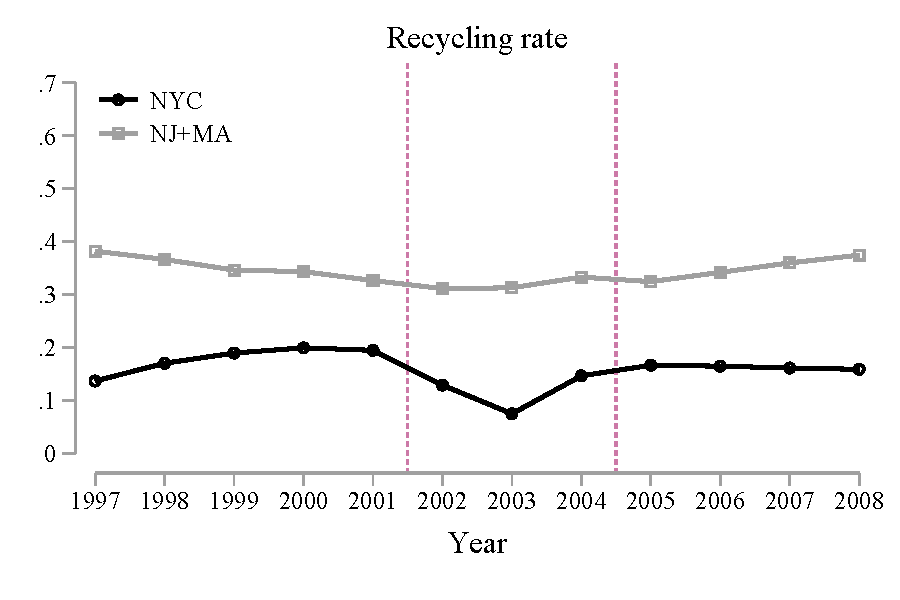
\includegraphics[width=0.7\textwidth]{./figure/recyclingrate.pdf}
    \caption{Treatment vs Control}
    \label{f:treatment_vs_control} 
\end{figure}

\item Using a TWFE regression, the average treatment effect is -0.06198 with a standard error of 0.00582.

\item Using SDID commad, the average treatment effect is -0.06436 with a standard error of 0.00679.
\begin{figure}[H]
    \centering
    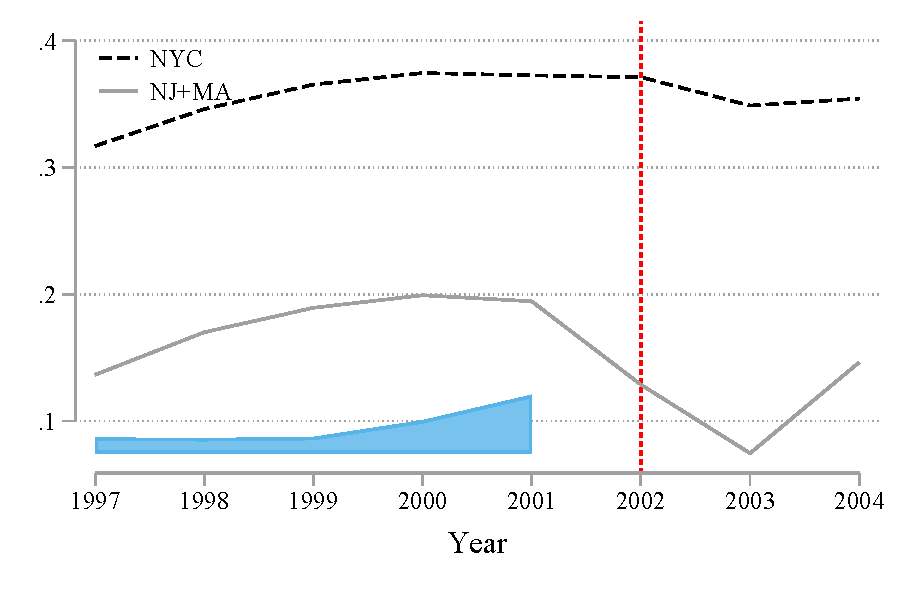
\includegraphics[width=0.7\textwidth]{./figure/sdid.pdf}
    \caption{Synthetic DID Plot}
    \label{f:sdid} 
\end{figure}

\item Event study plot
\begin{figure}[H]
    \centering
    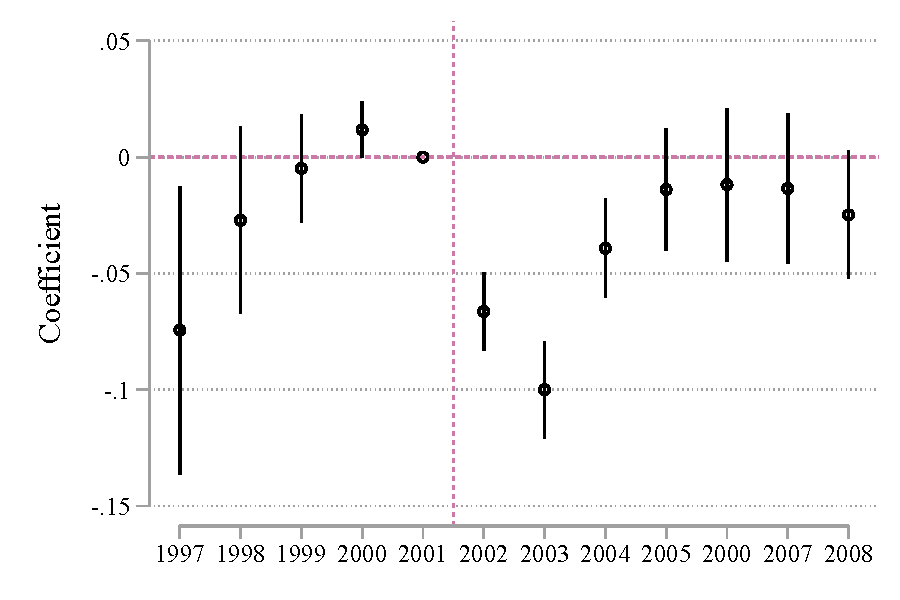
\includegraphics[width=0.7\textwidth]{./figure/eventstudy.pdf}
    \caption{Event Study Plot}
    \label{f:event} 
\end{figure}

\item Synthetic Control, graph style following Brewer and Cameron (2023)'s replication code.
\begin{enumerate}
    \item Raw outcomes for treatment and controls
    \begin{figure}[H]
        \centering
        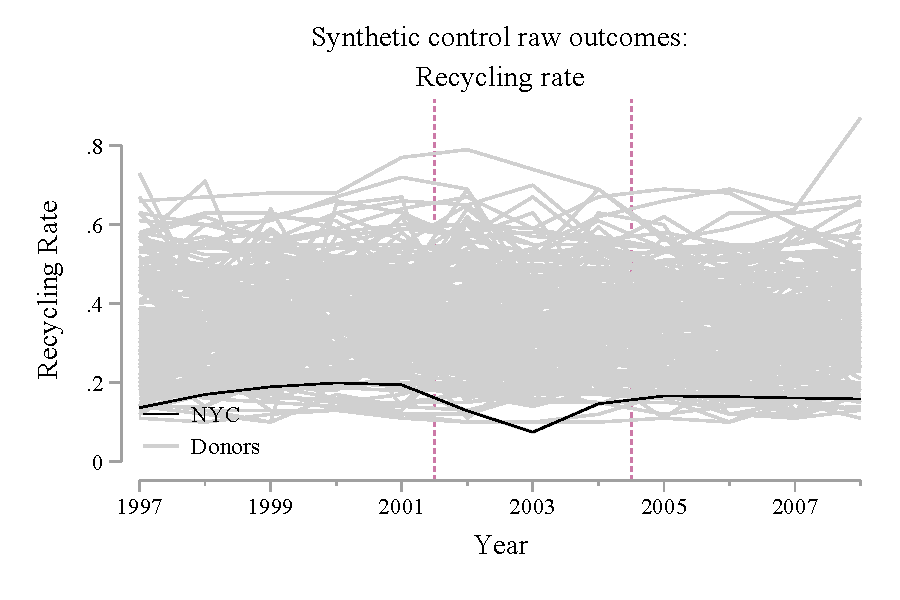
\includegraphics[width=0.7\textwidth]{./figure/raw.pdf}
        \caption{Raw outcomes for treatment and controls}
        \label{f:raw}
    \end{figure}
    \item Raw outcomes for treatment and synthetic control
    \begin{figure}[H]
        \centering
        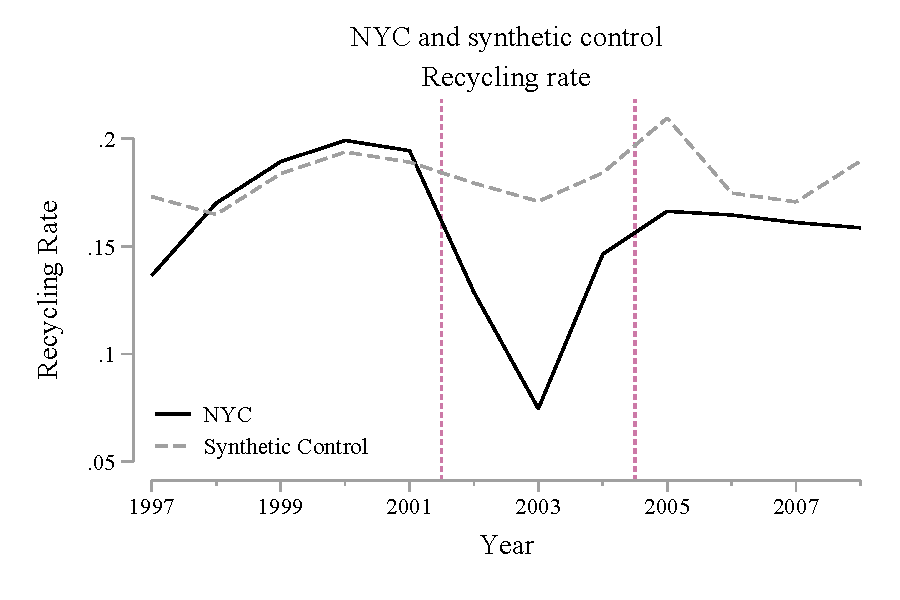
\includegraphics[width=0.7\textwidth]{./figure/treatmentcontrol.pdf}
        \caption{Raw outcomes for treatment and synthetic control}
        \label{f:tvsc}
    \end{figure}
    \item Estimated synthetic control effects and placebo effects
    \begin{figure}[H]
        \centering
        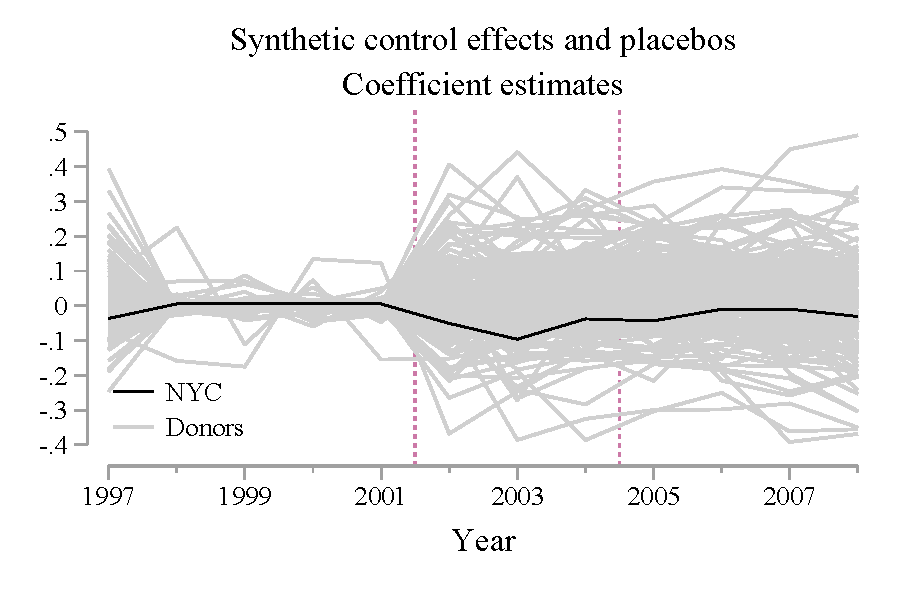
\includegraphics[width=0.7\textwidth]{./figure/placebo.pdf}
        \caption{Estimated synthetic control effects and placebo effects}
        \label{f:placebo}
    \end{figure}
    \item Synthetic control estimates
    \begin{figure}[H]
        \centering
        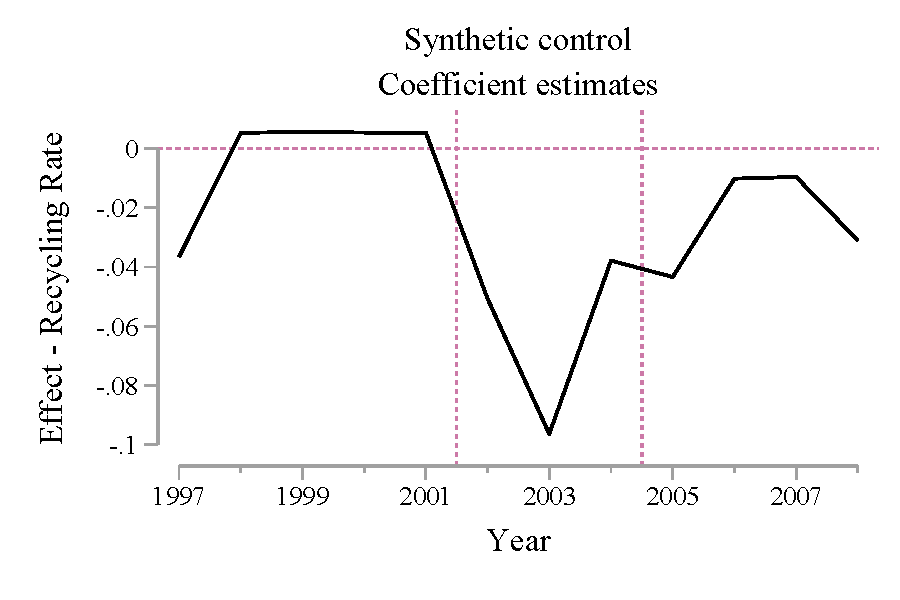
\includegraphics[width=0.7\textwidth]{./figure/effect.pdf}
        \caption{Estimated synthetic control effects and placebo effects}
        \label{f:effect}
    \end{figure}
\end{enumerate}


\end{enumerate}



\end{document}